\documentclass{article}

\usepackage{ctex}
\usepackage{amsfonts}
\usepackage{amsmath}
\usepackage{amsthm}
\usepackage{graphicx}
\usepackage{float}
\usepackage{hyperref}
\usepackage{mathabx}
\usepackage{datetime}
\usepackage{tabularray}
\usepackage{mathrsfs}
\usepackage{geometry}
\usepackage{wrapfig}

\title{普通物理学}
\author{}
\date{\today}

\geometry{a4paper,scale=0.8}

\begin{document}

\hypersetup{
    hidelinks,
    %colorlinks = true,
    allcolors = black,
    %pdfstartview = Fit,
    breaklinks = true
}

\newtheorem{definition}{Definition}[subsubsection]
\newtheorem{theorem}{Theorem}[subsubsection]
\newtheorem{corollary}{Corollary}[theorem]
\renewcommand{\proofname}{\indent\bf Proof}
\numberwithin{equation}{subsection}

\def\d{\mathrm d}
\def\scre{\mathscr E}

\newcommand{\bs}[1]{\boldsymbol{#1}}
\newcommand{\p}[1]{\left(#1\right)}

\begin{titlepage}
    \maketitle
\end{titlepage}

\tableofcontents
\newpage

\section{常数}

\begin{center}
    \begin{tblr}{c|c|c|c}
        \hline
        常量                     & 符号            & 值                           & 量纲                 \\
        \hline
        地球重力加速度           & $g$             & $9.8$                        & $m/s^2$              \\
        圆周率                   & $\pi$           & $3.1415926\cdots$            &                      \\
        真空光速                 & $c$             & $2.99792458\cdot{10}^8$      & $m/s$                \\
        绝对零度                 &                 & $0\p{-273.15^{\circ}C}$      & $K$                  \\
        元电荷                   & $e$             & $1.602117733\cdot{10}^{-19}$ & $C$                  \\
        引力常量                 & $G$             & $6.672\cdot{10}^{-11}$       & $N\cdot m^2/{kg}^2$  \\
        静电力常量               & $k$             & $8.987551\cdot{10}^9$        & $N\cdot m^2/C^2$     \\
        真空介电常量             & $\varepsilon_0$ & $8.854187817\cdot{10}^{-12}$ & $C^2/\p{N\cdot m^2}$ \\
        真空磁导率               & $\mu_0$         & $4\pi\cdot{10}^{-7}$         & $T\cdot m/A$         \\
        阿伏伽德罗常数           & $N_A$           & $6.0221367\cdot{10}^{23}$    & $mol^{-1}$           \\
        普朗克常数               & $h$             & $6.62607015\cdot{10}^{-34}$  & $J\cdot s$           \\
        里德伯常量               & $R$             & $1.097373157\cdot{10}^7$     & $m^{-1}$             \\
        气体摩尔体积(标准情况) & $n$             & $22.4$                       & $L/mol$              \\
        普适气体常数             & $R$             & $8.31$                       & $J/\p{mol\cdot K}$   \\
        玻尔兹曼常数             & $k_B$           & $1.380649\cdot{10}^{-23}$    & $J/K$                \\
        \hline
    \end{tblr}
\end{center}


\section{平动与转动}

\begin{enumerate}
    \item[$r$] 为某点到参考点的位矢
\end{enumerate}

\begin{center}
    \begin{tblr}{c|c|c||c|c|c}
        \hline
        \SetCell[c=3]{c}平动 &         &                         & \SetCell[c=3]{c}转动 &             &                             \\
        \hline
        位移                 & $\bs x$ &                         & 角度                 & $\theta$    &                             \\
        速度                 & $\bs v$ & $\dfrac{\d\bs x}{\d t}$ & 角速度               & $\bs\omega$ & $\dfrac{\d\theta}{\d t}$    \\
        加速度               & $\bs a$ & $\dfrac{\d\bs v}{\d t}$ & 角加速度             & $\bs\alpha$ & $\dfrac{\d\bs\omega}{\d t}$ \\
        质量                 & $m$     &                         & 转动惯量             & $J$         & $\displaystyle\int r^2\d m$ \\
        力                   & $\bs F$ & $m\bs a$                & 力矩                 & $\bs M$     & $J\bs\alpha=r\times\bs F$   \\
        动量                 & $\bs p$ & $m\bs v$                & 角动量               & $\bs L$     & $J\bs\omega=r\times\bs p$   \\
        冲量                 & $\bs I$ & $\bs Ft=\bs p-\bs p_0$  & 冲量矩               & $\bs H$     & $\bs Mt=\bs L-\bs L_0$      \\
        平动动能             & $E_k$   & $\dfrac12m\bs v^2$      & 转动动能             & $E_k$       & $\dfrac12J\bs \omega^2$     \\
        功                   & $A$     & $\bs F\bs x$            & 功                   & $A$         & $\bs M\theta$               \\
        \hline
    \end{tblr}
\end{center}

\section{能量}

\subsection{圆周运动}

\begin{enumerate}
    \item[$a_t$] 切向加速度
    \item[$a_n$] 法向加速度
\end{enumerate}

\[\bs v=R\bs\omega\]

\[\bs a_t=R\bs\alpha\]

\[\bs a_n=\frac{\bs v^2}R=\bs v\bs\omega=R\bs\omega^2\]

\subsection{保守力}

\begin{enumerate}
    \item[$k$] 弹性系数
\end{enumerate}

\[\oint\bs F\d\bs r=0\]

\begin{center}
    \begin{tblr}{c|c|c}
        \hline
        保守力类型 & 力$F/N$            & 势能$E_p/J$    \\
        \hline
        重力       & $mg$               & $mgh$          \\
        弹力       & $kx$               & $\dfrac12kx^2$ \\
        引力       & $G\dfrac{Mm}{r^2}$ & $G\dfrac{Mm}r$ \\
        电场
        力         & $k\dfrac{Qq}{r^2}$ & $k\dfrac{Qq}r$ \\
        \hline
    \end{tblr}
\end{center}

\subsection{动能}

\[E_k=\frac12mv^2=\frac{p^2}{2m}\]

\section{相对论}

\begin{enumerate}
    \item[$u$] 参考系移动速度,沿$Ox$方向
\end{enumerate}

\subsection{洛伦兹因子}

\[\gamma=\frac1{\sqrt{1-\p{\dfrac vc}^2}}\]

\subsection{相对论效应}

\begin{center}
    \begin{tblr}{c|c}
        \hline
        效应     & 表达式                \\
        \hline
        尺缩效应 & $l=\dfrac{l_0}\gamma$ \\
        钟慢效应 & $t=t_0\gamma$         \\
        质增效应 & $m=m_0\gamma$         \\
        \hline
    \end{tblr}
\end{center}

\subsection{质能方程}

\[E=mc^2\]

\subsection{静能}

\begin{enumerate}
    \item[$m_0$] 静质量
\end{enumerate}

\[E_0=m_0c^2\]

\subsection{洛伦兹变换}

\[\left\{\begin{aligned}
        x^\prime & =\p{x-ut}\gamma            \\
        t^\prime & =\p{t-\frac u{c^2}x}\gamma
    \end{aligned}\right.\]

\subsection{一维速度叠加}

\[v_x^\prime=\frac{v_x-u}{1-\dfrac u{c^2}v}\]

\subsection{相对论动量和能量关系式}

\[E^2=c^2p^2+E_0^2\]

\section{气体动理论}

\subsection{理想气体物态方程}

\begin{enumerate}
    \item[$p$] 气体压强
    \item[$V$] 气体体积
    \item[$T$] 气体热力学温度
    \item[$R$] 普适气体常数
    \item[$M$] 气体摩尔质量
    \item[$m$] 气体质量
\end{enumerate}

\[\frac{pV}T=\frac mMR\]

\begin{enumerate}
    \item[$n$] 单位体积内的气体分子数
    \item[$k_B$] 玻尔兹曼常数,$k_B=\dfrac R{N_A}$
\end{enumerate}

\[p=nk_BT\]

\subsection{压强}

\begin{enumerate}
    \item[$\bar\varepsilon_{tk}$] 分子平均平动动能
\end{enumerate}

\[p=\frac23n\bar\varepsilon_{tk}\]

\subsection{气体分子方均根速率}

\[v_{rms}=\sqrt{\bar{v^2}}=\sqrt{\frac{3k_BT}{m_0}}=\sqrt{\frac{3RT}M}\]

\subsection{能量按自由度均分定理}

\begin{enumerate}
    \item[$i$] 气体分子自由度
\end{enumerate}

\[\bar\varepsilon_k=\frac i2k_BT\]

\begin{center}
    \begin{tblr}{c|c|c|c}
        \hline
        分子类型       & 平动自由度$i_t$ & 转动自由度$i_r$ & 分子平均总动能$\bar\varepsilon_k$ \\
        \hline
        单原子分子     & 3               & 0               & $\dfrac 32k_BT$                   \\
        刚性双原子分子 & 3               & 2               & $\dfrac 52k_BT$                   \\
        刚性多原子分子 & 3               & 3               & $3k_BT$                           \\
        非刚性分子     & 3               & >1              & 还有振动自由度等                  \\
        \hline
    \end{tblr}
\end{center}

\subsection{内能}

\[E=\frac mM\frac i2RT=\frac {mN_A}M\bar\varepsilon_k\]

\subsection{气体分子速率分布函数}

\[f\p{v}=\frac{\d N}{N\d v}\]

\subsubsection{归一化条件}

\[\int\limits_0^{+\infty}f\p{v}\d v=1\]

可据此求出

\[\Delta N=N\int_{v_1}^{v_2}f\p{v}\d v\]

\[\Delta\bar v=\dfrac{\int_{v_1}^{v_2}vNf\p{v}\d v}{\Delta N}\]

\[\bar v=\int\limits_0^{+\infty}vf\p{v}\d v\]

\[\bar{v^2}=\int\limits_0^{+\infty}v^2f\p{v}\d v\]

\subsubsection{麦克斯韦速率分布律}

\begin{enumerate}
    \item[$m_0$] 单个气体分子质量
\end{enumerate}

\[f\p{v}=4\pi{\p{\frac{m_0}{2\pi k_BT}}}^{\frac32}\exp\p{-\frac{m_0v^2}{2k_BT}}v^2\]

\subsection{平均自由程}

\begin{enumerate}
    \item[$\bar v$] 算术平均速率
    \item[$\bar Z$] 碰撞频率
    \item[$d$] 分子的作用球半径
    \item[$n$] 单位体积内的气体分子数
\end{enumerate}

\[\bar\lambda=\frac{\bar v}{\bar Z}=\frac1{\sqrt2\pi d^2n}\]

\section{热力学}

\subsection{热力学第一定律}

\begin{enumerate}
    \item[$Q$] 吸收热量
    \item[$\Delta E$] 内能增量
    \item[$A$] 对外做功
\end{enumerate}

\[Q=\Delta E+A\]

\subsection{准静态过程}

\begin{enumerate}
    \item[$C_m$] 摩尔热容
    \item[$C_{V,m}$] 气体的摩尔定容热容,$C_{V,m}=\dfrac i2R$
    \item[$C_{p,m}$] 气体的摩尔定压热容(迈耶公式),$C_{p,m}=C_{V,m}+R$
    \item[$C_{p,m}$] 气体的摩尔多方热容,$C_{,m}=C_{V,m}+\frac R{1-n}$
    \item[$\gamma$] 摩尔热容比,$\gamma=\dfrac{C_{p,m}}{C_{V,m}}=\dfrac{i+2}i$
    \item[$n$] 多方指数,$1<n<\gamma$,且:
        \[n=\left\{\begin{aligned}
                \infty &  & \text{等容过程} \\
                0      &  & \text{等压过程} \\
                1      &  & \text{等温过程} \\
                \gamma &  & \text{绝热过程} \\
            \end{aligned}\right.\]
\end{enumerate}

\begin{longtblr}[
        caption = {热力学},
        remark{注} = {在微分形式下$\Delta$变为微分算子$\d$}
    ]{colspec={c|c|c|c|c|c|c},hlines}
    过程 & 常量       & 过程方程(常量)              & $A$                                                                              & $Q$                                         & $\Delta E$                 & $C_m$     \\
    等容 & $V$        & $pT^{-1}$                     & 0                                                                                & \SetCell[c=2]{c} $\dfrac mMC_{V,m}\Delta T$ &                            & $C_{V,m}$ \\
    等压 & $p$        & $VT^{-1}$                     & $p\Delta V=\dfrac mMR\Delta T$                                                   & $\dfrac mMC_{p,m}\Delta T$                  & $\dfrac mMC_{V,m}\Delta T$ & $C_{p,m}$ \\
    等温 & $T$        & $pV$                          & \SetCell[c=2]{c} $\dfrac mMRT\ln\dfrac{V_2}{V_1}=\dfrac mMRT\ln\dfrac{p_1}{p_2}$ &                                             & $0$                        & $\infty$  \\
    绝热 & $\delta Q$ & $\begin{aligned}
                                  & pV^\gamma               \\
                                  & V^{\gamma-1}T           \\
                                  & p^{\gamma-1}T^{-\gamma}
                             \end{aligned}$ & $\begin{aligned}
                                                     & -\dfrac mMC_{V,m}\Delta T       \\
                                                   = & -\dfrac{\Delta\p{pV}}{\gamma-1}
                                               \end{aligned}$                             & $0$                                         & $\dfrac mMC_{V,m}\Delta T$ & $0$                                                          \\
    多方 &            & $\begin{aligned}
                                  & pV^n          \\
                                  & V^{n-1}T      \\
                                  & p^{n-1}T^{-n}
                             \end{aligned}$           & $\begin{aligned}
                                                              & \dfrac mMRT\ln\dfrac{V_2}{V_1}=               \\
                                                              & \dfrac mMRT\ln\dfrac{p_1}{p_2}  & \p{n=1}     \\
                                                              & -\dfrac{\Delta\p{pV}}{n-1}      & \p{n\neq 1}
                                                         \end{aligned}$                & $A+\Delta E$                                & $\dfrac mMC_{V,m}\Delta T$ & $C_{n,m}$                                                       \\
\end{longtblr}

\subsection{循环过程}

若$p-V$坐标轴上有默认顺时针的循环过程$C$,即

\[\Delta E=0\]

\[A=Q_1-Q_2=\oint_C\d V\]

\subsubsection{热机效率}

\begin{enumerate}
    \item[$Q_1$] 从高温热源吸收热量
    \item[$Q_2$] 向低温热源放出热量
\end{enumerate}

\[\eta=\frac A{Q_1}=\frac{Q_1-Q_2}{Q_1}\]

\[A=Q_1-Q_2=\oint_C\d V\]

若为逆时针即为制冷(积分为负)

\subsubsection{制冷系数}

\begin{enumerate}
    \item[$Q_1$] 向高温热源放出热量
    \item[$Q_2$] 从低温热源吸收热量
\end{enumerate}

\[w=\frac {Q_2}A=\frac{Q_2}{Q_1-Q_2}\]

\subsubsection{卡诺循环}

两个绝热和两个等温过程组成的循环

\begin{enumerate}
    \item[$T_1$] 高温热源
    \item[$T_2$] 低温热源
\end{enumerate}

\[\eta_C=\frac{Q_1-Q_2}{Q_1}=1-\frac{T_1-T_2}{T_1}\]

\[w_C=\frac{Q_2}{Q_1-Q_2}=\frac{T_2}{T_1-T_2}\]

\subsection{熵}

在可逆过程中

\[\oint\frac{\delta Q}T=0\]

\[\d S=\frac{\delta Q}T\]

\[\Delta S_{1\to2}=\int_{1\to2}\frac{\delta Q}T\]

\subsubsection{自由膨胀不可逆}

\subsubsection{玻尔兹曼关系}

\begin{enumerate}
    \item[$W$] 热力学概率
\end{enumerate}

\[S=k_B\ln W\]

\section{静电场}

\subsection{库仑定律}

\begin{enumerate}
    \item[$\bs F$] 试探电荷受到的库仑力
    \item[$Q$] 场源电荷
    \item[$q$] 试探电荷
    \item[$r$] 两电荷间距
    \item[$\varepsilon_0$] 真空介电常量
    \item[$k$] 静电力常量
    \item[$\bs e$] 场源电荷到试探电荷的方向
\end{enumerate}

\[\bs F=\frac1{4\pi\varepsilon_0}\frac{Qq}{r^2}\bs e=k\frac{Qq}{r^2}\bs e\]

\subsection{电场强度}

\[\bs E=\frac{\bs F}q=\frac Q{4\pi\varepsilon_0r^2}\bs e\]

\subsection{电场强度通量}

\[\bs\Psi_E=\bs E\cdot\bs S\]

\subsection{高斯定理(有源场)}

\[\Psi_E=\oiint_S\bs E\cdot\d\bs S\]

\paragraph{点电荷$q$为球心的球壳上通量为}

\[\Psi_E=\frac q{\varepsilon_0}\]

\subsection{环路定理(无旋场)}

\[\oint\bs E\cdot\d\bs l=0\]

\subsection{电势能}

取无限远处为电势零点

\begin{enumerate}
    \item[$r$] 距离电荷$r$处
\end{enumerate}

\[W=q\int\limits_r^{+\infty}\bs E\cdot\d\bs l\]

\subsection{电势}

\[V=\frac Wq=\int\limits_r^{+\infty}\bs E\cdot\d\bs l=\frac Q{4\pi\varepsilon_0r}\]

\[V=\frac q{4\pi\varepsilon_0r}\]

\[U=\Delta V\]

\subsection{微分关系}

\[\nabla V=\frac{\d V}{\d n}\bs e_n=-\bs E\]

\subsection{静电平衡}

闭合曲面导体内,电荷分布在导体外表面上,内部无电荷分布

\begin{enumerate}
    \item[$\sigma$] 电荷的面密度
    \item[$\bs e_n$] 面的法向量
\end{enumerate}

\[\bs E=\frac\sigma{\varepsilon_0}\bs e_n\]

\subsection{常见导体总结}

\begin{enumerate}
    \item[$q$] 总电荷量
    \item[$r$] 球心到样点距离
    \item[$\lambda$] 电荷线密度
    \item[$\sigma$] 电荷面密度
    \item[$r_0$] 电势零点
\end{enumerate}

\begin{longtblr}[
        caption = {静电场},
        remark{注} = {壳内部电场为0,电势同壳}
    ]{colspec={c|c|c},hlines}
    均匀带电导体类型 & 场强$E$                             & 电势$V$                                           \\
    球壳             & $\dfrac q{4\pi\varepsilon_0r^2}$    & $\dfrac q{4\pi\varepsilon_0r}$                    \\
    无限长圆柱面     & $\dfrac\lambda{2\pi\varepsilon_0r}$ & $\dfrac\lambda{2\pi\varepsilon_0}\ln\dfrac{r_0}r$ \\
    无限大平面       & $\dfrac\sigma{2\varepsilon_0}$      & $\dfrac\sigma{2\varepsilon_0}\p{r_0-r}$           \\
\end{longtblr}

\subsection{电容}

\paragraph{孤立导体的电容}

\[C=\frac QU\]

\subsubsection{相对介电常量}

\begin{enumerate}
    \item[$C_0$] 极板间为真空时的电容
\end{enumerate}

\[\varepsilon_r=\frac C{C_0}\]

\subsubsection{介电常量}

\[\varepsilon=\varepsilon_0\varepsilon_r\]

\subsubsection{串联}

\[\frac1C=\sum\frac1C_i\]

\subsubsection{并联}

\[C=\sum C_i\]

\subsubsection{电场能量}

\begin{enumerate}
    \item[$V$] 极板间体积
\end{enumerate}

\[W=\frac12CU^2=\frac12\varepsilon E^2V\]

\subsubsection{能量密度}

\[w_e=\frac WV=\frac12\varepsilon E^2\]

\subsubsection{常见电容总结}

\begin{enumerate}
    \item[$r$] 球心到样点距离
    \item[$R_1,R_2$] 圆柱(球)形电容半径
    \item[$l$] 圆柱长度
    \item[$d$] 极板间距(圆柱形电容中$d=R_2-R_1$)
    \item[$S$] 极板正对面积
\end{enumerate}

\begin{center}
    \begin{tblr}{colspec={c|c},hlines}
        电容类型   & 电容$C$                                          \\
        球形电容   & $4\pi\varepsilon r\p{\dfrac1{R_1}-\dfrac1{R_2}}$ \\
        圆柱形电容 & $\dfrac{2\pi\varepsilon l}{\ln R_2-\ln R_1}$     \\
        平行板电容 & $\varepsilon\dfrac Sd$                           \\
    \end{tblr}
\end{center}

\subsection{电介质}

\begin{enumerate}
    \item [$\bs D$] 电位移
    \item [$\bs P$] 电极化强度
\end{enumerate}

\[\bs D=\varepsilon_0\bs E+\bs P=\varepsilon\bs E\]

\subsubsection{有电介质时的高斯定理}

\[\oiint_S\bs D\cdot\d\bs S=q_0\]

\section{恒定电流的磁场}

\subsection{电流}

\[I=\frac{\d q}{\d t}\]

\subsection{电流密度}

\begin{enumerate}
    \item[$S$] 垂直于电流的截面面积
\end{enumerate}

\[\bs j=\frac{\d I}{\d S}\]

\subsection{电动势}

\begin{enumerate}
    \item [$E_k$] 非静电性场的场强
\end{enumerate}

\[\scre=\frac{\d A}{\d q}=\int_B^A\bs E_k\cdot\d\bs l=\oint_L\bs E_k\cdot\d\bs l\]

\subsection{欧姆定律}

\[R=\frac VI=\rho\frac lS\]

\subsection{磁感应强度和磁通量}

\subsubsection{磁感应强度}

\[B=\frac{\d\Phi}{\d S}\]

\subsubsection{磁通量}

\[\Phi=\int_L\bs B\cdot\d\bs S\]

\subsection{毕奥-萨伐尔定律}

电流元对某点激发的磁场

\begin{enumerate}
    \item [$\mu_0$] 真空磁导率
    \item [$r$] 电流元到某点的距离
    \item [$e_r$] 从电流元指向某点的单位向量
\end{enumerate}

\[\d\bs B=\frac{\mu_0}{4\pi}\frac{I\d\bs l\times\bs e_r}{r^2}\]

\[\bs B=\frac{\mu_0}{4\pi}\int_L\frac{I\d\bs l\times\bs e_r}{r^2}\]

\subsection{运动电荷磁场}

一个电荷运动产生的磁场

\begin{enumerate}
    \item [$\bs v$] 电荷运动速度
\end{enumerate}

\[I=nqvS\]

\[\d N=nS\d\bs l\]

\[\bs B_q=\frac{\d\bs B}{\d N}=\frac{\mu_0}{4\pi}\frac{q\bs v\times\bs e_r}{r^2}\]

\subsection{恒定磁场高斯定理(无源场)}

\[\oiint\limits_S\bs B\cdot\d\bs S=0\]

\subsection{安培环路定理(有旋场)}

\[\oint_L\bs B\cdot\d\bs l=\mu_0\sum I\]

\subsection{霍尔效应}

\begin{figure}[H]
    \centering
    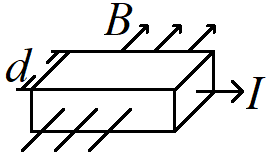
\includegraphics[width=0.2\linewidth]{HallEffect.png}
\end{figure}

\begin{enumerate}
    \item [$U$] 霍尔电势差
    \item [$R_H$] 霍尔系数
\end{enumerate}

\[U=R_H\frac{IB}d=\frac{IB}{nqd}\]

\[R_H=\frac1{nq}\]

\subsection{安培力}

弗莱明右手定则

\begin{enumerate}
    \item [$\bs e_I$] 电流方向向量
\end{enumerate}

\[\bs F=IL\bs e_I\times\bs B\]

\subsection{磁场对载流线圈的作用}

\begin{enumerate}
    \item [$\bs m$] 磁矩
    \item [$N$] 线圈匝数
    \item [$S$] 线圈面积
    \item [$\bs M$] 磁力矩
\end{enumerate}

\[m=NIS\]

\[\bs M=\bs m\times\bs B\]

\subsection{磁场力做功}

\[A=I\Delta\Phi\]

\subsection{洛伦兹力}

弗莱明右手定则

\[\bs F=q\bs v\times\bs B\]

\subsection{磁介质}

\begin{enumerate}
    \item [$\bs H$] 磁场强度
    \item [$\bs M$] 磁化强度
\end{enumerate}

\[\bs B=\mu_0\p{\bs H+\bs M}=\mu\bs H\]

\subsubsection{有磁介质时的安培环路定理}

\[\oint\bs H\cdot\d\bs l=\sum I\]

\section{电磁感应}

\subsection{法拉第电磁感应定律}

\subsubsection{磁通链}

\begin{enumerate}
    \item [$N$] 线圈匝数
\end{enumerate}

\[\Psi=N\Phi\]

\subsubsection{感应电动势}

\[\scre_i=-\frac{\d\Psi}{\d t}=-N\frac{\d\Phi}{\d t}\]

\subsubsection{感应电流}

\[I_i=\frac{\scre_i}R\]

\subsubsection{感应电荷}

\[q=\int_{t_1}^{t_2}I_i\d t=\frac{\Delta\Phi}R\]

\subsection{动生电动势}

\[\scre=\p{-\bs v\times\bs B}\cdot\bs l=\p{\bs B\times\bs v}\cdot\bs l\]

\subsection{运动导线内部电场}

\[\bs E_k=\bs v\times\bs B\]

\subsection{感生电场(有旋无源场)}

\begin{enumerate}
    \item [$\bs E_i$] 感生电场强度
\end{enumerate}

\[\oint_L\bs E_i\cdot\d\bs l=-\iint_S\frac{\partial\bs B}{\partial t}\cdot\d\bs S\]

\[\oiint_S\bs E_i\cdot\d\bs S=0\]

\subsection{自感和互感}

\subsubsection{自感应}

\begin{enumerate}
    \item [$L$] 自感系数
\end{enumerate}

\[L=\frac{\Psi}I=\mu_0\frac{N^2}l\pi R^2\]

\[\scre_L=-L\frac{\d I}{\d t}\]

\subsubsection{互感应}

\begin{enumerate}
    \item [$L$] 互感系数
    \item [$k$] $\in\left[0,1\right]$ 耦合因数
\end{enumerate}

\[M=\frac{\Phi_{21}}{I_1}=\frac{\Phi_{12}}{I_2}=k\sqrt{L_1L_2}\]

\[\begin{aligned}
        \scre_{21} & =-M\frac{\d I_1}{\d t} \\
        \scre_{12} & =-M\frac{\d I_2}{\d t}
    \end{aligned}\]

\subsection{磁场能量}

\[W_m=\frac12LI_0^2=\frac12I\Psi\]

\subsection{能量密度}

\begin{enumerate}
    \item [$\mu$] 磁导率
\end{enumerate}

\[w_m=\frac{W_m}V=\frac{B^2}{2\mu}=\frac12\bs B\cdot\bs H\]

\subsection{位移电流}

\begin{enumerate}
    \item [$I_d$] 位移电流
    \item [$j_d$] 位移电流密度
\end{enumerate}

\[I_d=S\frac{\d D}{\d t}=\frac{\d\Psi}{\d t}\]

\[j_d=\frac1S\frac{\d\Psi}{\d t}=\frac{\d D}{\d t}\]

\[\oint_L\bs H\cdot\d\bs l=\sum\p{I+I_d}=\int_S\bs j\cdot\d\bs S+\int_S\frac{\partial\bs D}{\partial t}\cdot\d\bs S\]

\subsection{麦克斯韦方程组}

\[\left\{\begin{aligned}
         & \oiint_S\bs D\cdot\d\bs S=\sum q=\iiint_V\rho\d V                                                           \\
         & \oiint\limits_S\bs B\cdot\d\bs S=0                                                                          \\
         & \oint_L\bs E\cdot\d\bs l=-\frac{\d\Psi}{\d t}=-\iint_S\frac{\partial\bs B}{\partial t}\cdot\d\bs S          \\
         & \oint_L\bs H\cdot\d\bs l=I+I_d=\iint_S\bs j\cdot\d\bs S+\iint_S\frac{\partial\bs D}{\partial t}\cdot\d\bs S \\
    \end{aligned}\right.\]

\end{document}
